\documentclass{astroedu-lab}

\begin{document}

\pagestyle{plain}

\begin{problem}{\huge Лабораторная работа 5.2.2\\\\Изучение спектров атомов водорода\\\\и молекул йода\\\\Выполнил Жданов Елисей Б01-205}

\section{Цель работы:}

1) Провести измерения спектров водорода и йода

2) Определить постоянную Ридберга и характеристики молекул.

\section{Оборудование:}

Монохроматор

Коллиматор

Неоновая и ртутная лампы

Водородная лампа

Кювета с кристаллами йода и лампа накаливания на штативе


\section{Теоретическая справка}
	
	\paragraph{Спектр атомов водорода.}
	
	Объяснение структуры спектра излучения атомов требует решения задачи о движении электрона в эффективном поле атома.	Для атома водорода и водородоподобных (одноэлектронных) атомов 	определение энергетических уровней значительно упрощается, так как	квантово-механическая задача об относительном движении электрона (заряд $ -e $, масса $ m_e $) и ядра (заряд $ Z_e $, масса $ M $) сводится к задаче о движении частицы с эффективной массой $ \mu = m_e M /(m_e+M) $ в кулоновском поле $ - Z \varepsilon^2 / n $. Длины волн спектральных линий водородоподобного атома описываются формулой
	\begin{equation}\label{key}
		\dfrac{1}{\lambda_{m n}} = R Z^2 \left(\dfrac{1}{n^2}-\dfrac{1}{m^2}\right),
	\end{equation}
	где $ m, \;n \in \mathbb{Z} $, а $ R $ -- постоянная Ридберга.
	Эта формула позволяет по энергиям перехода судить о расположении энергетических уровней атома водорода. На рис. \ref{fig:screenshot1} изображены энергетические уровни и соответствующие им переходы, определяющие спектр.
	\begin{wrapfigure}{}{0.5\textwidth}
		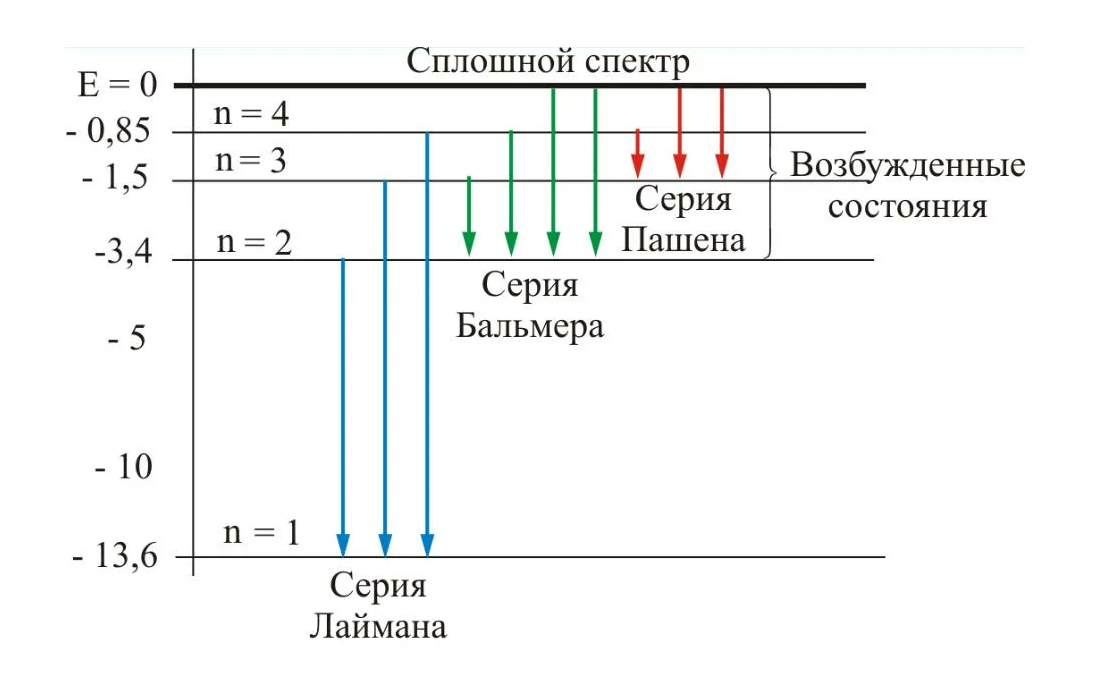
\includegraphics[width=1.0\linewidth]{Screenshot_1}
		\caption{Энергетические уровни атома водорода}
		\label{fig:screenshot1}
	\end{wrapfigure}
	В данной работе изучается серия Бальмера, линии которой лежат в видимой области. Для серии Бальмера $ n = 2 $. Величина $ m $ для первых четырех линий этой серии принимает значение 3, 4, 5, 6. Эти линии	обозначаются символами $ H_\alpha,\;H_\beta,\;H_\gamma,\;H_\delta $.
	
	Оценим энергии основного и возбужденного состояний водородоподобного атома. Чтобы найти основное состояние квантовой системы, надо минимизировать, с учетом соотношения неопределенностей, полную энергию. Потенциальная энергия электрона равна кулоновской энергии электрона в поле ядра с зарядом $ Z e $. Так как электрон локализован в области размером $ r $, то его импульс $ p \simeq \hbar / r $, и полная энергия определяется выражением
	\begin{equation}\label{eq:energy}
		E = \dfrac{-Z e^2}{r}+\dfrac{\hbar^2}{2 m_e r^2}.
	\end{equation}
	Приняв за нуль производную этого выражения, получим
	\begin{equation*}\label{key}
		r_\text{Б} = \dfrac{\hbar^2}{Z m_e e^2}.
	\end{equation*}
	Это значение радиуса первой орбиты для электрона в поле ядра с зарядом $ Z $ -- боровского радиуса. Подставляя в \eqref{eq:energy} это значение, получим
	\begin{equation*}\label{key}
		E = -R Z^2,
	\end{equation*}
	\begin{equation}\label{key}
		R = \dfrac{m_e e^4}{2 \hbar^2}.
	\end{equation}
	Для возбуждённых состояний значения энергий можно найти аналогично, приняв во внимание, что $ p \simeq n \hbar / r $ из условия, что на длине орбиты укладывается целое число волн де Бройля. Отсюда энергия $ n $-го уровня равна 
	\begin{equation*}\label{key}
		E = \dfrac{-R Z^2}{n^2}.
	\end{equation*}
	
	\paragraph{Спектр молекул йода.}
	
	\begin{wrapfigure}{}{0.5\textwidth}
		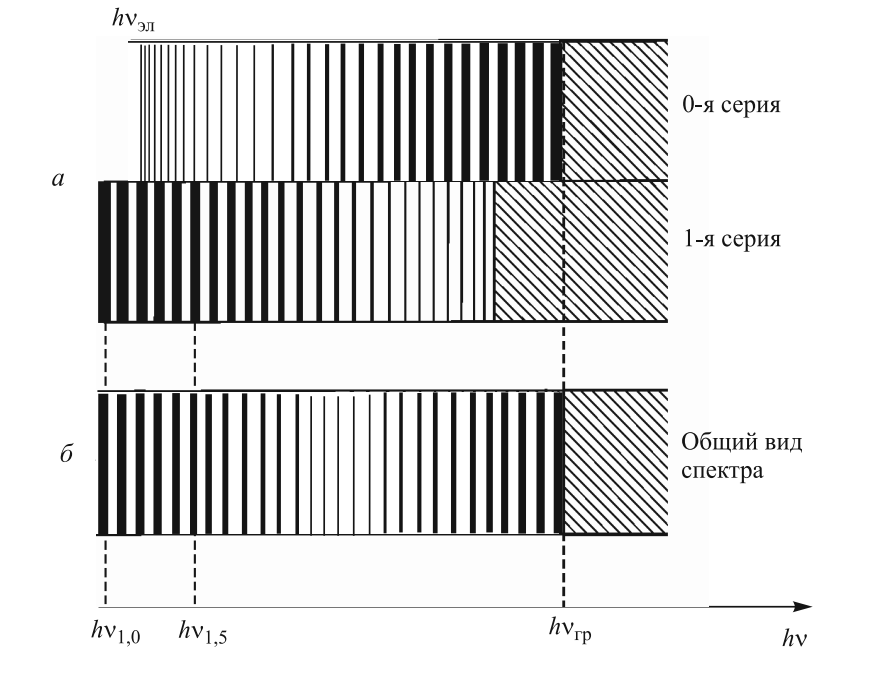
\includegraphics[width=1.0\linewidth]{Screenshot_3}
		\caption{Спектральная картина йода}
		\label{fig:screenshot3}
	\end{wrapfigure} 
	Массы ядер атомов велики по сравнению с массой электрона. Благодаря такой разнице в массах, скорости движения ядер в молекуле малы по сравнению со скоростями электронов. Это даёт возможность	рассматривать электронное движение при неподвижных ядрах, расположенных на определенных расстояниях друг от друга. Определяя уровни энергии такой системы, мы найдем электронные термы молекул. Любой атом в молекуле находится в электрическом поле остальных ее атомов. Оно вызывает расщепление электронных уровней атомов в молекуле. Следует отметить, что при соединении атомов в молекулу заполненные оболочки атомов мало меняются. Существенно может измениться распределение электронной плотности в не до конца заполненных оболочках.
	
	
	Спектр молекулярного йода представлен на рис. \ref{fig:screenshot3}.
	Для расчёта спектра поглощения йода необходимо учесть энергии колебательного и вращательного движения молекул. Видимый спектр состоит из 0-й и 1-й серий Деландра. 2-я серия в 10 раз менее интенсивная, чем 0-я, и поэтому ей пренебрегаем. 
	
	Энергетическое	положение линий поглощения описывается выражением
	\begin{equation}\label{eq:йод}
		h \nu_{0 n_2} = (E_2 - E_1 )+ h \nu_2 \left(n_2+\dfrac{1}{2}\right) - \dfrac{1}{2}h \nu_1.
	\end{equation}
%	\begin{wrapfigure}{}{0.3\textwidth}
%		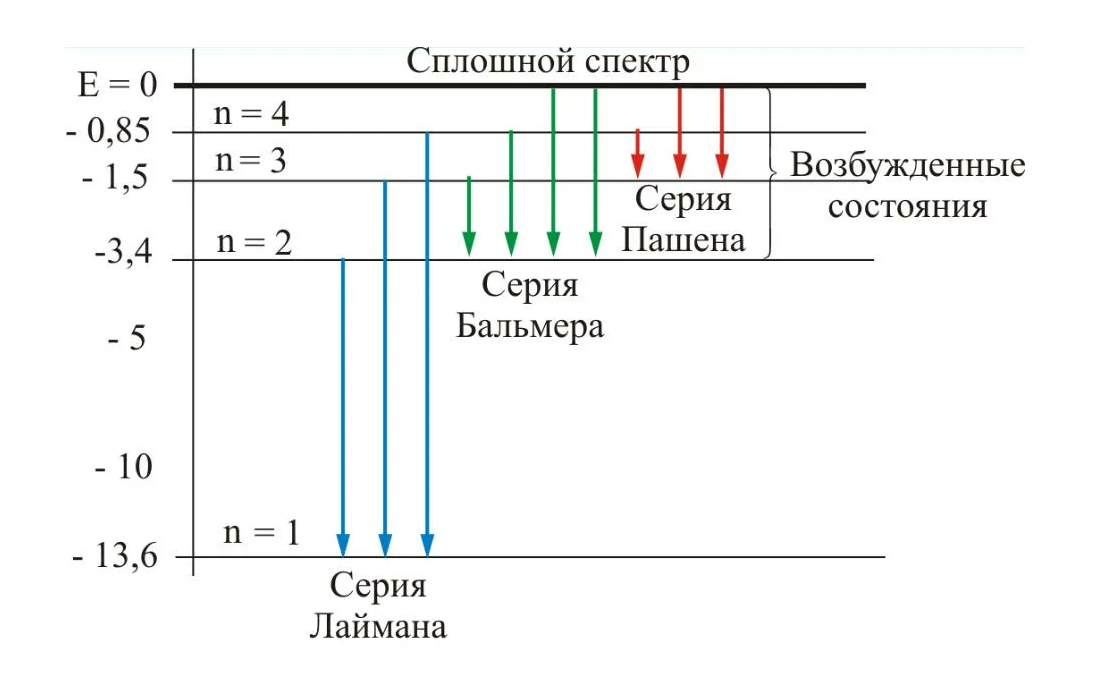
\includegraphics[width=1.0\linewidth]{Screenshot_1}
%		\caption{Энергетические уровни атома водорода}
%		\label{fig:screenshot1}
%	\end{wrapfigure}

\newpage

		
\section{Экспериментальная установка}
	
	\begin{figure}[!h]
		\centering
		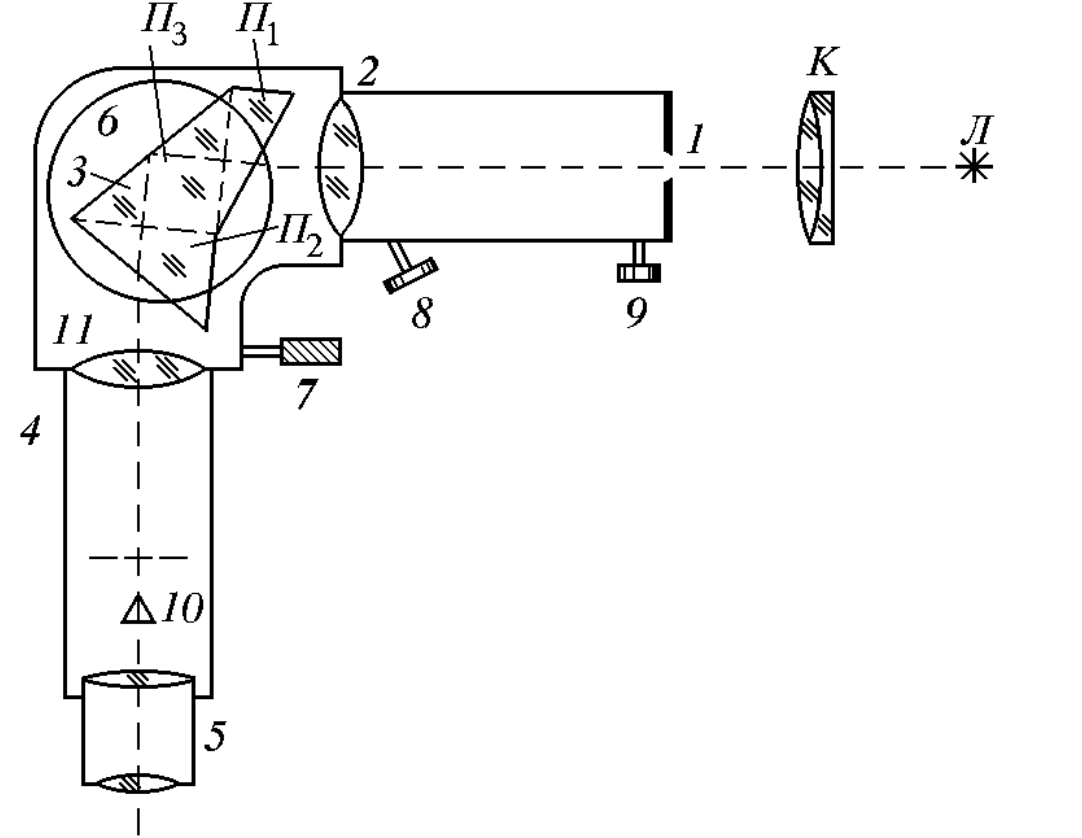
\includegraphics[width=0.6\textwidth]{Screenshot_2}
		\caption{Схема монохроматора}
		\label{fig:screenshot2}
	\end{figure}
	
.

Установка состоит из монохроматора, который предварительно калибруется и направляющей, на которую устанавливаются соответствующие источники излучения.

\section{Измерения, Обработка}

\subsection{Калибровка}
	
	Построим калибровочный график по спектрам неона и ртути на рис. 4. Зависимость нелинейная, но аппроксимируется полиномом второй степени:
	
	\begin{figure}[!h]
		\centering
		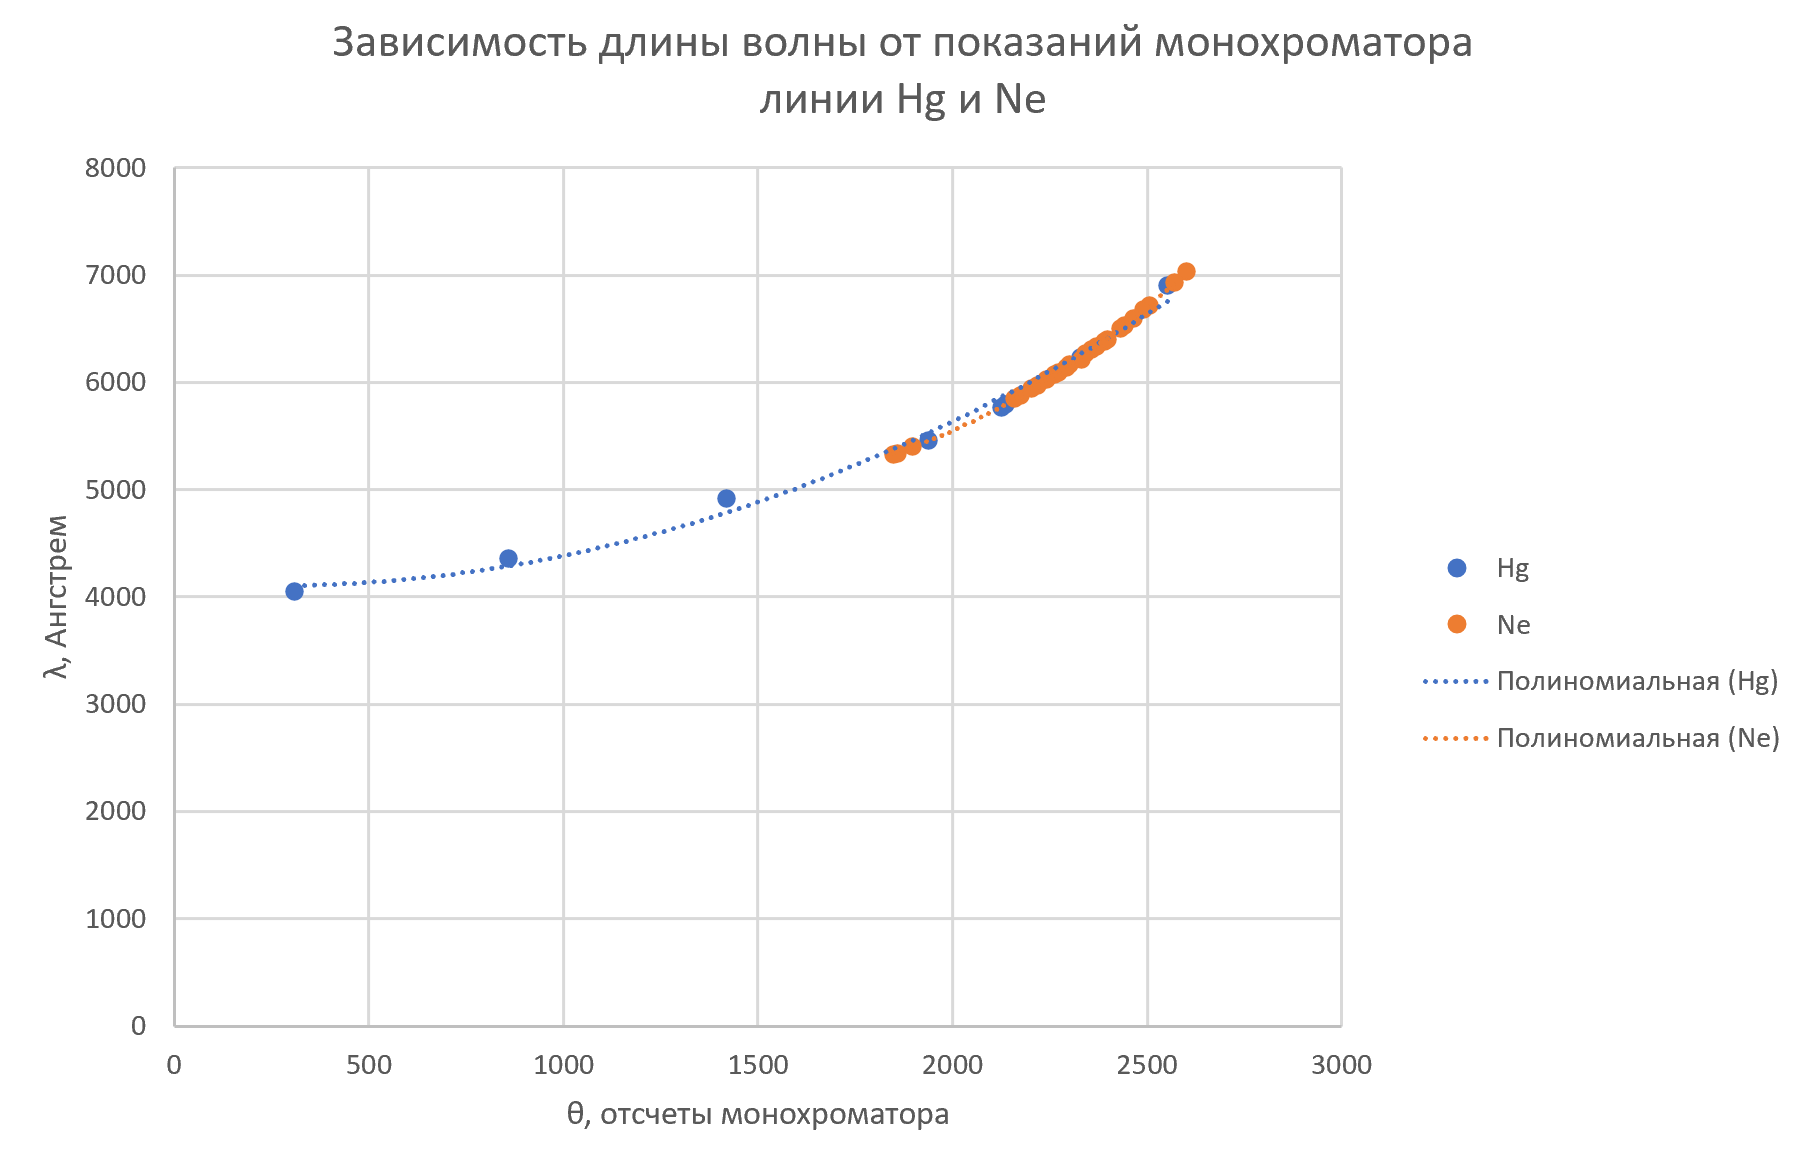
\includegraphics[width=0.9\linewidth]{nehg}
		\caption{Калибровочный график по линиям водорода и йода}
		\label{fig:graph1}
	\end{figure}
	
	Для сравнения на рис. 5 приведена общая аппроксимация точек. Как видно, кривые для ртути и неона немного не совпадают, что просто учесть, вписав отличие в погрешность.
	
	\begin{figure}[!h]
		\centering
		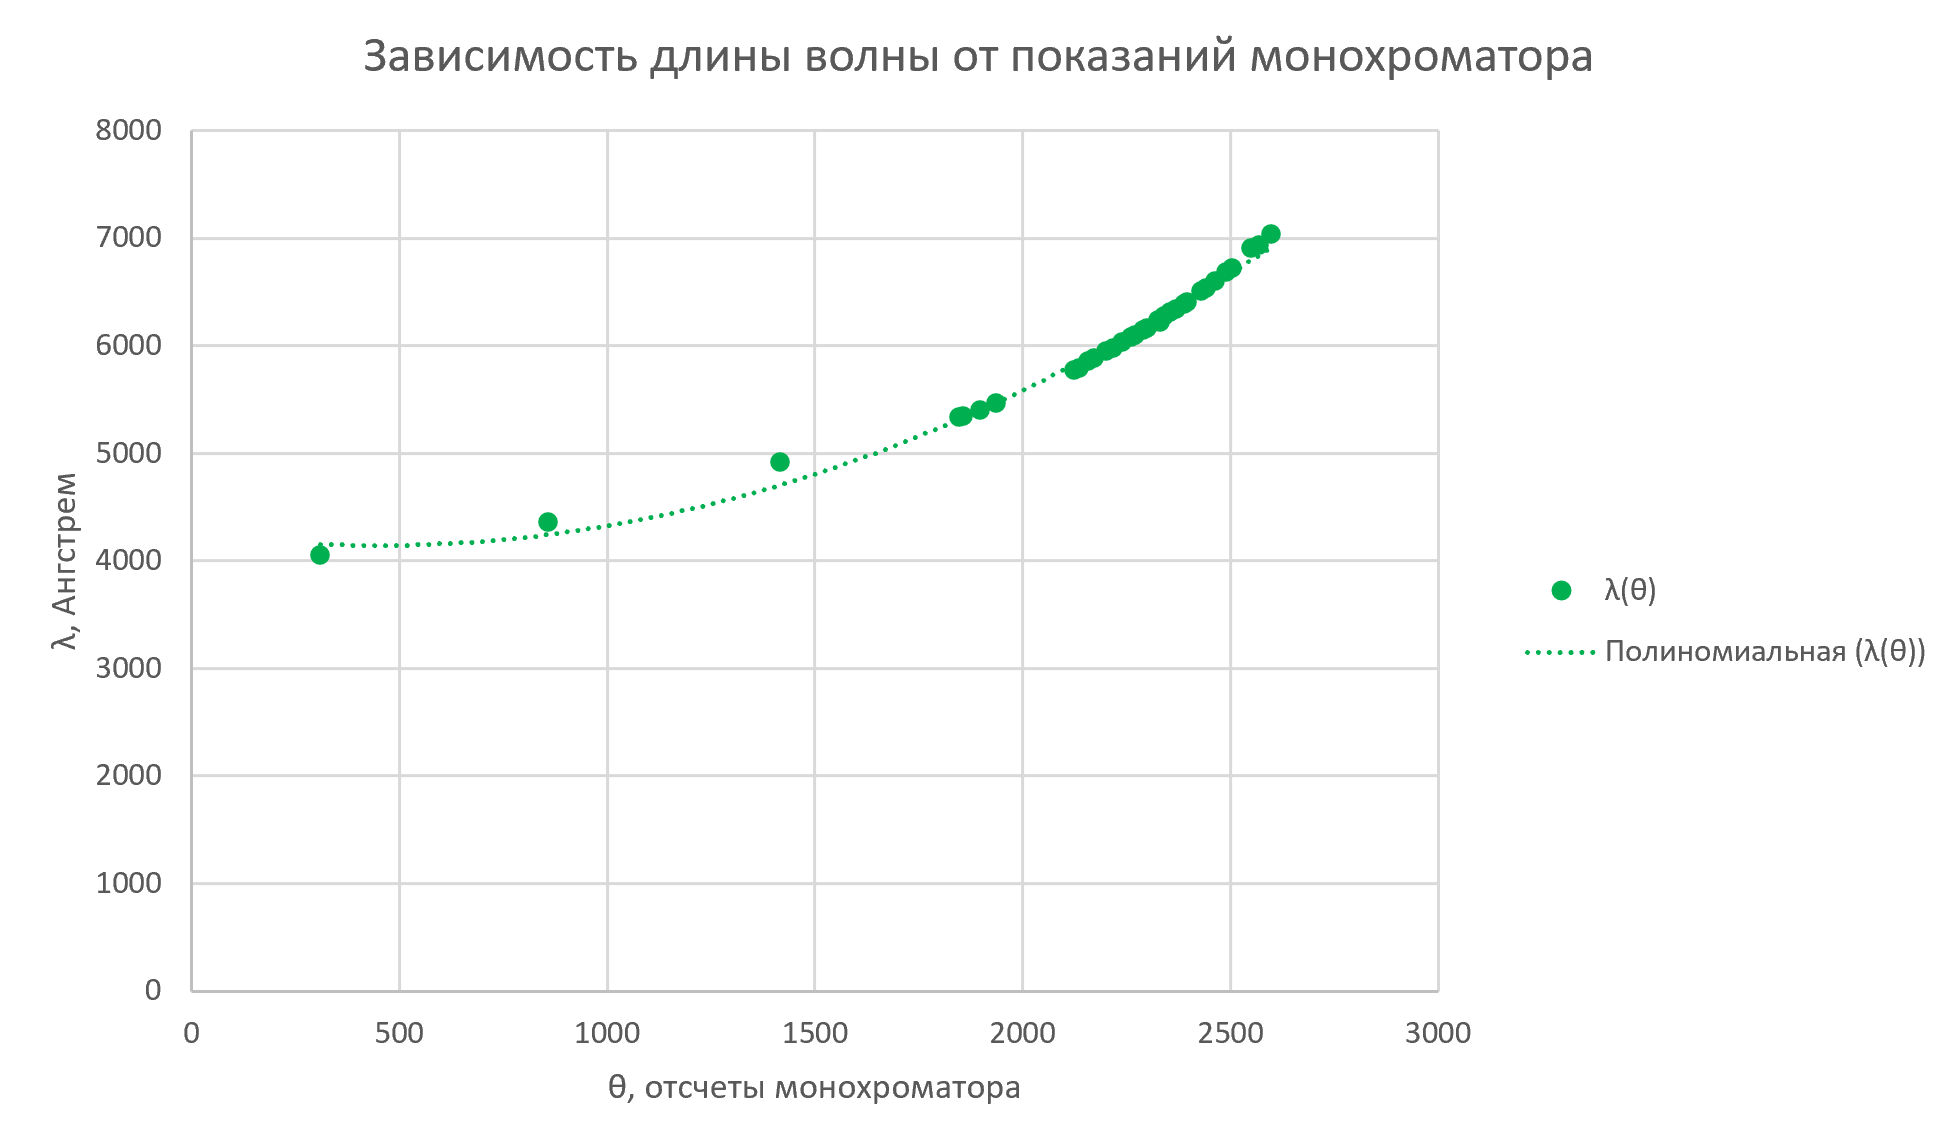
\includegraphics[width=0.9\linewidth]{int}
		\caption{Калибровочный график по всем линиям}
		\label{fig:graph2}
	\end{figure}
	
Итак, полученные аппроксимационные уравнения


\[
y=0.0006 \cdot x^2 - 0.54 \cdot x + 4260
\]

Средняя ошибка аппроксимации: 0.8 $\%$

На такие значения и будем опираться.

\newpage
	
\subsection{Исследование спектров}
	
	Определим длины волн $H_\alpha,\;H_\beta,\;H_\gamma,\;H_\delta $ при помощи полученной калибровочной формулы. Результаты в табл. \ref{tab:H}:
	\begin{table}[h]
		\centering
		\begin{tabular}{|l|l|l|}
			\hline
			& $\theta^\circ$ & $\lambda, A$ \\ \hline
			$ H_\alpha$ & $2452\pm 2$      & $6570\pm 50$        \\ \hline
			$H_\beta$   & $1468\pm 2$      & $4840\pm 40$         \\ \hline
			$H_\gamma$  & $826\pm 2$      & $4310\pm 30$         \\ \hline
			$H_\delta$  & $412\pm 2$       & $4110\pm 30$         \\ \hline
		\end{tabular}
		\caption{Спектральные линии водорода}
		\label{tab:H}
	\end{table}
	В пределах погрешности полученные значения совпадают с табличными для серии Бальмера. Определим постоянную Ридберга. Построим график зависимости $ \lambda^{-1} $ от выражения вида $ 1/2^2 - 1/m^2 $ на рис.
	\begin{figure}[!h]
		\centering
		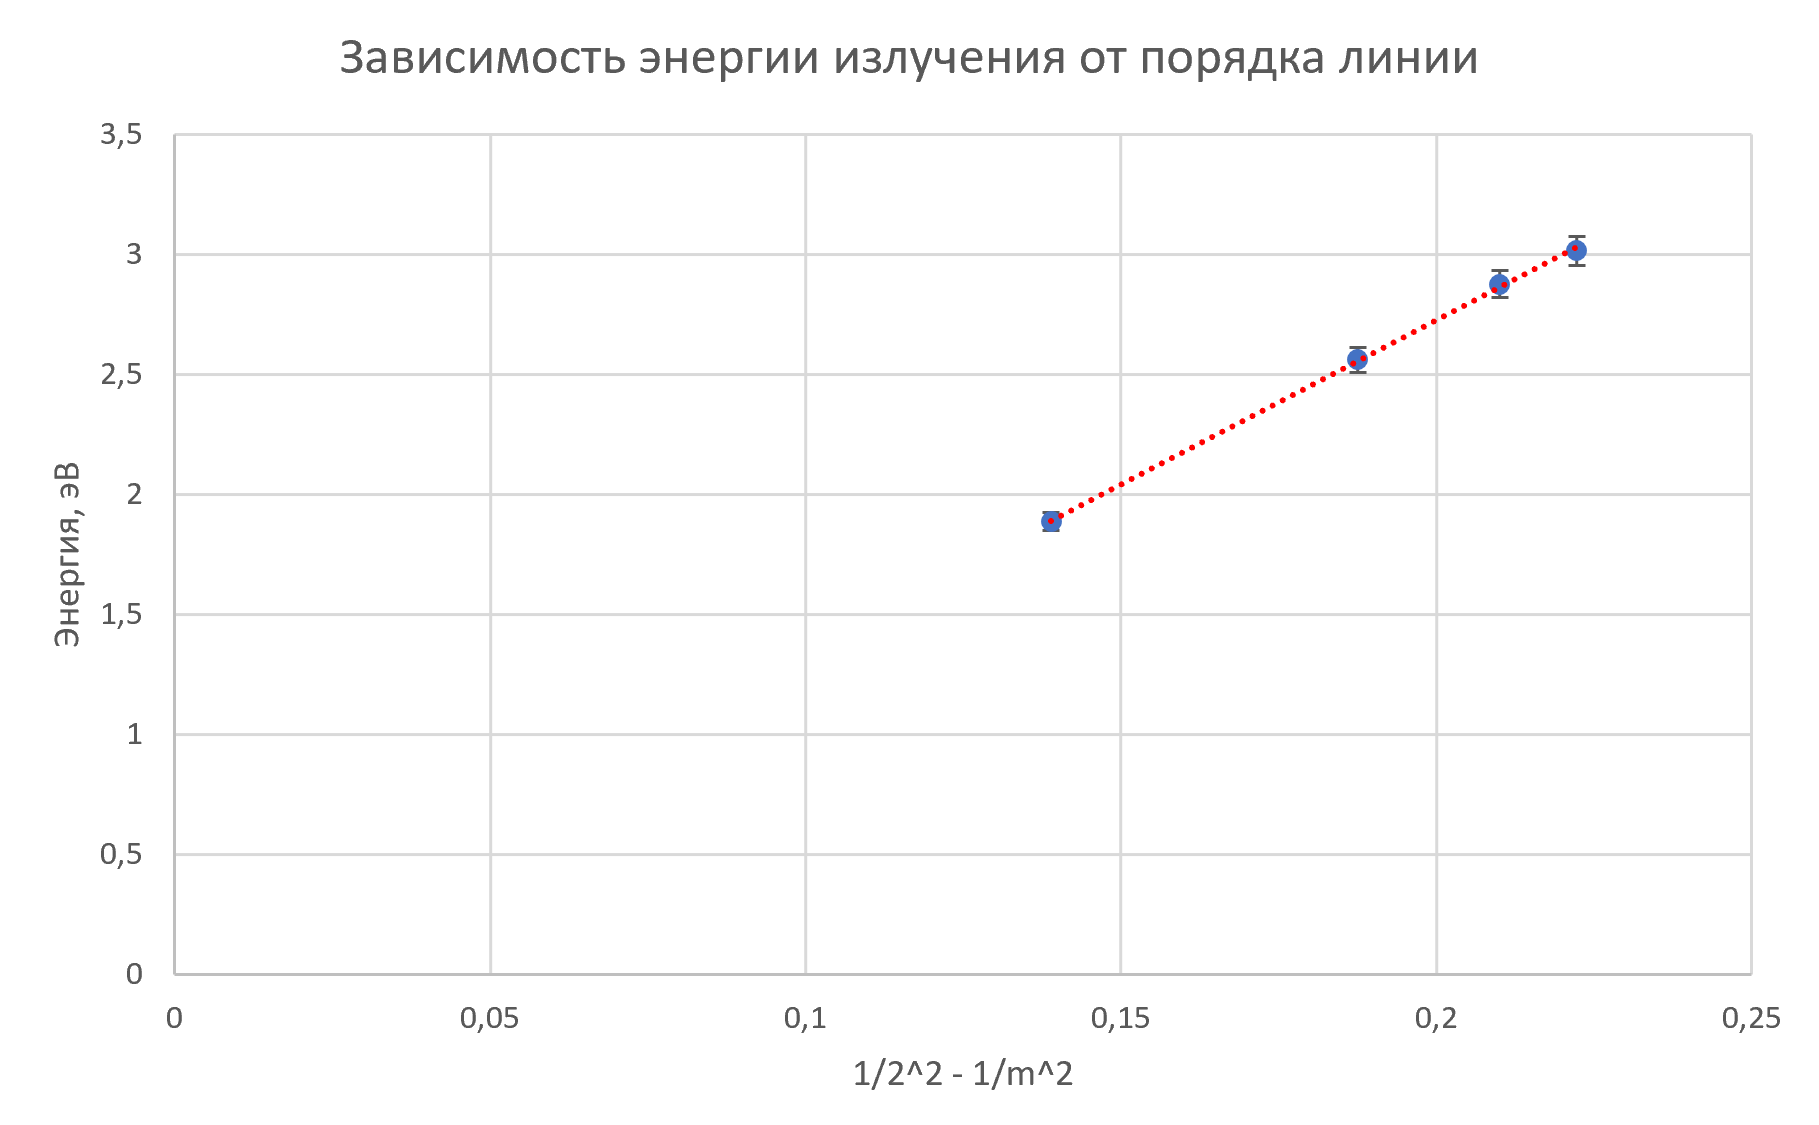
\includegraphics[width=0.9\linewidth]{R}
		\caption{Калибровочный график по всем линиям}
		\label{fig:graph2}
	\end{figure}

Найдем угловые коэффициенты прямых для каждой установки по МНК.

\[
	a = \frac{<x_i y_i> - < x > < y_i >}{< x_i^2> - < x_i >^2}
\]

\[
	b = < \nu_i > - a < N_i >
\]

Также рассчитаем их погрешности

\begin{equation}
	S_a^2 = \frac{< x_i^2>}{< x_i^2 > - < x_i >^2} \cdot \frac{<  b_i - b > ^2}{n - 2}
\end{equation}

Уравнение прямой:

\begin{equation}
	y = (-0.008 \pm 0.044) + (13.67 \pm 0.23) \cdot x
\end{equation}

\begin{center}
	Красота, $R = 13.67 \pm 0.23$ эВ.
\end{center}
	
\newpage	
	
	Найдём длины волн для йода:
	\[\nu_{1, 0} = 6100\pm 50 A\]
	\[\nu_{1, 5} = 5880\pm 50 A\]
	\[\nu_{гр} = 5020\pm 40 A\]
	Вычислим в электрон-вольтах энергию колебательного кванта возбуждённого состояния молекулы йода:
	\[h\nu_2 = \frac{h\nu_{1, 5} - h\nu_{1, 0}}{5} = 15 \text{ мэВ}.\]
	
	Найдём параметры диссоциации молекул йода:
	\[h\nu_{\text{эл}} = h\nu_{1, 0}+\dfrac{3}{2}h\nu_1 - \dfrac{1}{2}h\nu_2 = 2.13\pm 0.03 \text{ эВ}.\]
	Эта величина получена из формулы \eqref{eq:йод}. Тогда для энергии диссоциации частиц в основном и возбуждённом состояниях:
	\[D_1 = h\nu_{гр} - E_A = 1.48\pm 0.02\text{ эВ},\]
	\[D_2 = h\nu_{гр} - h\nu_{\text{эл}} = 0.28\pm 0.02\text{ эВ}.\]
	Здесь $ E_A = 0.94 \text{ эВ}$ -- энергия возбуждения атома.


\section{Вывод}

Полученное значение постоянной Ридберга точно соответствует теории, что говорит о верной постановке эксперимента и не в последнюю очередь о точности спектрометрии. Полученные значения энергии диссоциации йода соответствуют теоретическим ожиданиям.


\section{Ресурсы}

Расчет по МНК: метод-наименьших-квадратов.рф

https://planetcalc.ru/8735/ - аппроксимация с погрешностью


\end{problem}
\end{document}